\chapter{測試案例分析}
本章節將為擴充的代理關鍵字撰寫單元測試\cite{ut},並且將改善翻譯邏輯與一詞多譯功能後的i18n工具,做功能的展示。最後將i18n工具套用至一個使用到多項代理關鍵字的Robot Framework測試腳本,以呈現“多國語言網頁自動化驗收測試”的效果。

%4.1
\section{新增與修改之代理關鍵字的單元測試}
以下將以Microsoft中文官方網頁\cite{microsoft},以及筆者使用Node.js\cite{nodejs}自行架設的i18n測試網頁(i18n Testing Website)為受測網站,為各個新增或已修改實作之代理關鍵字,分別提供Robot Framework的單元測試腳本,以驗證原生關鍵字在套用新的代理關鍵字下,能夠獨立正常運作。但為求精簡,本論文將不重複放上同類型關鍵字的測試腳本。(經修改的第一版i18n代理關鍵字前將加上‘*’標示)

%4.1.1
\subsection{Alert Should Be Present}
\begin{figure}[H]
\begin{lstlisting}[language={python}]
*** Settings ***
Library    SeleniumLibrary
Library    ../self_util.py
Test Setup    Run Keywords    Open Browser    http://localhost:3000    Chrome
...                    AND    Maximize Browser Window
Test Teardown    Close Browser

*** Test Cases ***
Alert should be present
    Wait until Element Is Visible    //*[normalize-space()='Show Alert Message']    timeout=${shortPeriodOfTime}
    Double Click Element    //*[normalize-space()='Show Alert Message']
    Alert Should Be Present    Welcome to Bing's website
\end{lstlisting}
\caption{Alert Should Be Present在代理關鍵字下執行的測試腳本}
\end{figure}
此測試腳本(如圖4.1)會打開i18n Testing Website,並雙擊Show Alert Message按鈕,使畫面跳出alert視窗(如圖4.2)。最後使用Alert Should Be Present來驗證alert資訊是否為“歡迎光臨Bing的網頁”。測試通過,代表參數“Welcome to Bing’s website”有成功被翻譯為“歡迎光臨Bing的網頁”(如圖4.3)。

\begin{figure}[H]
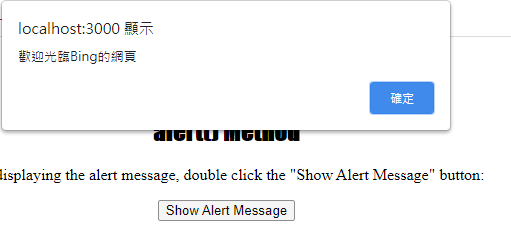
\includegraphics[width= \textwidth]{../論文截圖/4-1-2 alert視窗的文字.png}
\caption{網頁上的alert視窗顯示的文字}
\end{figure}

\begin{figure}[H]
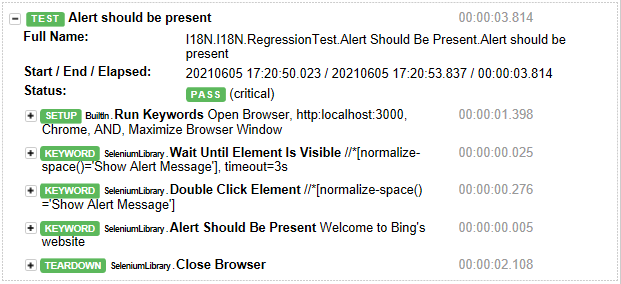
\includegraphics[width= \textwidth]{../論文截圖/4.1.1-3 pass.png}
\caption{Alert Should Be Equal測試通過}
\end{figure}

\hspace*{\fill} \\
\\ \hspace*{\fill} \\
\\ \hspace*{\fill} \\
\\ \hspace*{\fill} \\
\\ \hspace*{\fill} \\
%4.1.2
\subsection{Count Values In List}
\begin{figure}[H]
\begin{lstlisting}[language={python}]
*** Test Cases ***
Count values in list
    @{list1} =    Create List    支援    Software
    ${number} =    Count Values In List    ${list1}    Support
    Log    ${number}
\end{lstlisting}
\caption{Count Values In List在代理關鍵字下執行的測試腳本}
\end{figure}
此測試腳本(如圖4.4),一開始會利用Create List創出一個包含「支援」和‘Software’的list,並使用Count Values In List來計算參數‘Support’出現在此list中幾次。第一次執行測試通過(如圖4.5),透過Log印出的數字為1,代表參數‘Support’被翻譯為「支援」後,出現在list中一次,所以測試通過;且系統將支援當成“Support”翻譯的其中一種,並跳出一詞多譯UI。之後,使用者選擇「支援」作為唯一翻譯。第二次測試通過(如圖4.6),透過Log印出的數字為1,且不跳出一詞多譯UI與warning資訊。

\begin{figure}[H]
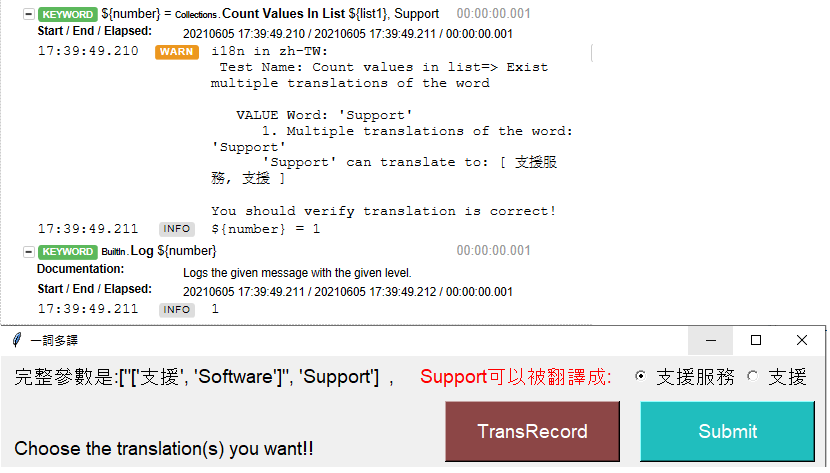
\includegraphics[width= \textwidth]{../論文截圖/4.1.2-2 count values in list 1st run.png}
\caption{Count Values In List測試腳本第一次執行通過}
\end{figure}

\begin{figure}[H]
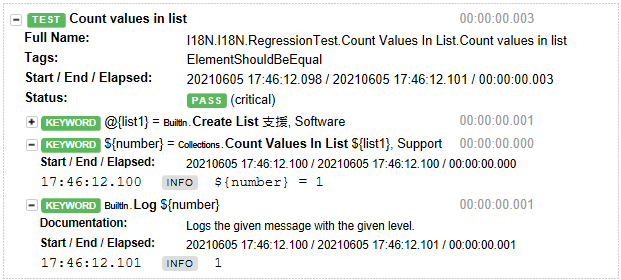
\includegraphics[width= \textwidth]{../論文截圖/4.1.2-3 count values in list 2nd run.png}
\caption{Count Values In List測試腳本第二次執行通過}
\end{figure}

\hspace*{\fill} \\
\\ \hspace*{\fill} \\
\\ \hspace*{\fill} \\
\\ \hspace*{\fill} \\
\\ \hspace*{\fill} \\
%4.1.3
\subsection{Dictionaries Should Be Equal}
\begin{figure}[H]
\begin{lstlisting}[language={python}]
*** Test Cases ***
Dictionaries should be equal
&{dict1} =    Create Dictionary    軟體=支援
&{dict2} =    Create Dictionary    Software=Support
Dictionaries Should Be Equal    ${dict1}    ${dict2}
\end{lstlisting}
\caption{Dictionaries Should Be Equal在代理關鍵字下執行的測試腳本}
\end{figure}
此測試腳本(如圖4.7),會利用Create Dictionary創出兩個dictionaries,分別是{'軟體': '支援'}和{'Software', 'Support'}(測試腳本的 ‘=’左側為key,右側為value),並使用Dictionaries Should Be Equal檢查兩者是否相同。第一次執行測試通過(如圖4.8),代表dictionary {‘Software’, ‘Support’}有成功被翻譯,且系統將“支援”當成“Support”翻譯的其中一種,並跳出一詞多譯UI。之後,使用者選擇“支援”作為唯一翻譯。第二次測試通過(如圖4.9),且不跳出一詞多譯UI與warning資訊,代表’Support’ 根據使用者選擇成功被翻譯為‘支援’。

\begin{figure}[H]
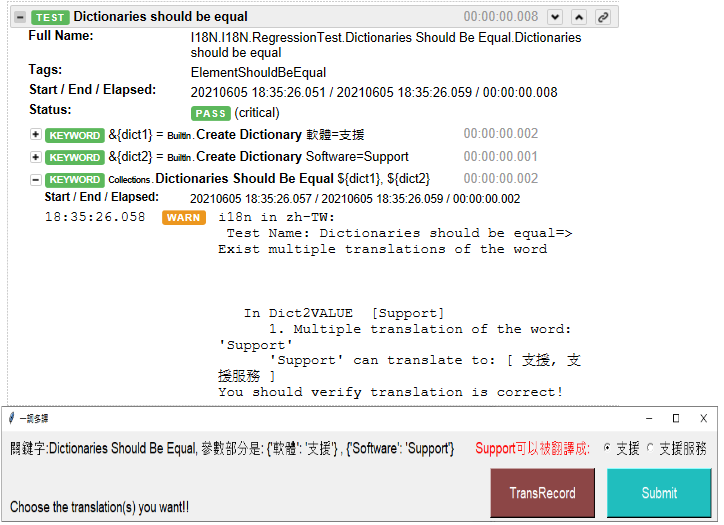
\includegraphics[width= \textwidth]{../論文截圖/4.1.3-2 dictionaries should be equal 1st run.png}
\caption{Dictionaries Should Be Equal測試腳本第一次執行通過}
\end{figure}

\begin{figure}[H]
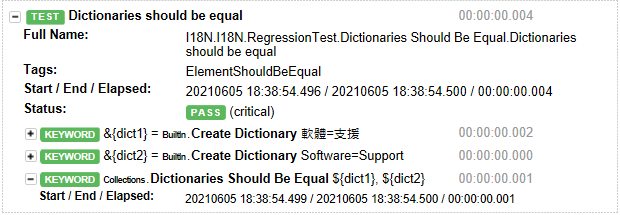
\includegraphics[width= \textwidth]{../論文截圖/4.1.3-3 dictionaries should be equal 2nd run.png}
\caption{Dictionaries Should Be Equal測試腳本第二次執行通過}
\end{figure}

%4.1.4
\subsection{Select From List By Label}
\begin{figure}[H]
\begin{lstlisting}[language={python}]
*** Settings ***
Resource    ../CommonVariables.txt
Library    SeleniumLibrary
Test Setup    Run Keywords    Open Browser    http://localhost:3000    Chrome
...                    AND    Maximize Browser Window
Test Teardown    Close Browser

*** Test Cases ***
Select from list by the label "Support"
${defaultSelection} =    Set Variable    //*[@id='i18n-selection-list']//*[text()='Software' and @selected]
${selectionList} =    Set Variable    //*[@id='i18n-selection-list']
Wait Until Element Is Visible    ${defaultSelection}    timeout=${shortPeriodOfTime}
Select From List By Label    ${selectionList}    Support
List Selection Should Be    ${selectionList}    Support
\end{lstlisting}
\caption{Select From List By Label在代理關鍵字下執行的測試腳本}
\end{figure}
此測試腳本(如圖4.10),會打開i18n Testing Website,並使用Select From List By Label選取畫面上selection list的Support選項(如圖4.11)。之後用List Selection Should Be驗證結果是否正確。第一次測試通過(如圖4.12),而畫面上選擇了‘支援’,代表參數Support有成功被翻譯,且系統將‘支援’當作‘Support’的其中一種翻譯,隨後跳出了一詞多譯UI。之後,使用者選擇了‘支援服務’當作Support的唯一翻譯。第二次測試腳本通過(如圖4.13),畫面上被選擇的selection list顯示‘支援服務’,代表參數‘Support’成功被翻譯為使用者前一次的選擇。

\begin{figure}[H]
\centering
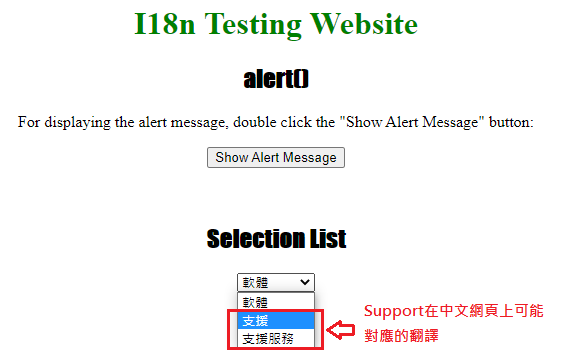
\includegraphics[width= .6\textwidth]{../論文截圖/4-1-7 Select from list by label要驗證的網頁元件.png}
\caption{Select From List By Label測試腳本要驗證的網頁元件}
\end{figure}

\begin{figure}[H]
\centering
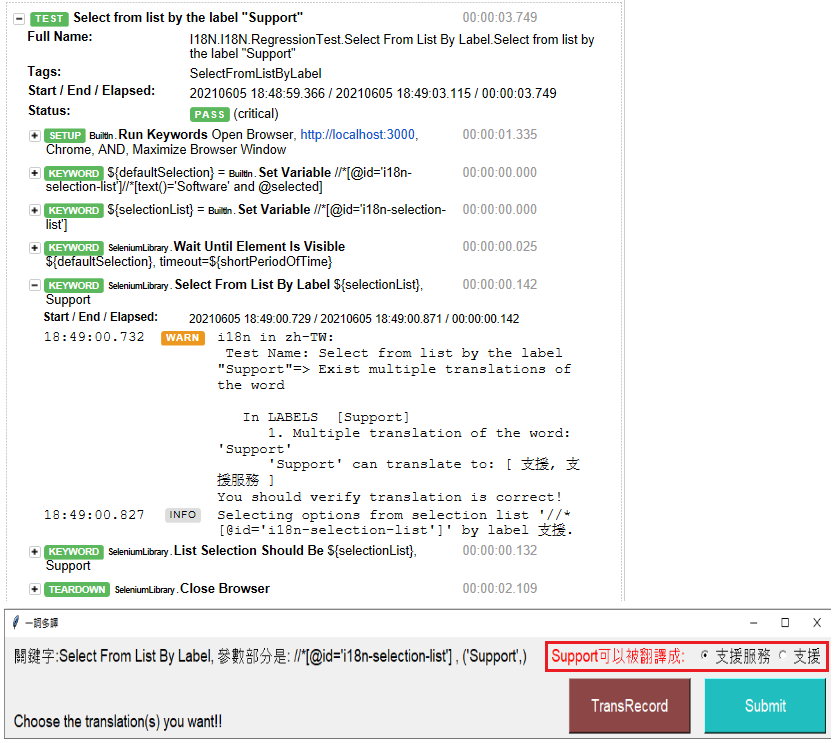
\includegraphics[width= .8\textwidth]{../論文截圖/4.1.4-2 select from list by label 1st run.png}
\caption{Select From List By Label測試腳本第一次執行通過}
\end{figure}

\begin{figure}[H]
\centering
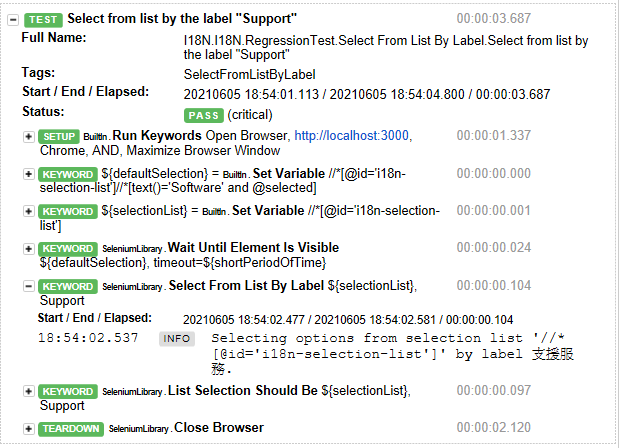
\includegraphics[width= .8\textwidth]{../論文截圖/4.1.4-3 select from list by label 2nd run.png}
\caption{Select From List By Label測試腳本第二次執行通過}
\end{figure}

\hspace*{\fill} \\
\\ \hspace*{\fill} \\
\\ \hspace*{\fill} \\
\\ \hspace*{\fill} \\
\\ \hspace*{\fill} \\
%4.1.5
\subsection{*Page Should Contain Element}
\begin{figure}[H]
\begin{lstlisting}[language={python}]
*** Settings ***
Resource    ../CommonVariables.txt
Library    SeleniumLibrary
Library    ../self_util.py
Test Setup    Run Keywords    Open Browser To Microsoft Page
...                    AND    Change Language    expectedLanguage=${language}
Test Teardown    Close Browser

*** Test Cases ***
Check "Microsoft Support" webelement is on the support page
    Go To Support Page
    ${MicrosoftSupport} =    Set Variable    //*[@id ='supHomeAndLandingPageHeaderContainer']//*[contains(text(), 'Support')]
    Page Should Contain Element    ${MicrosoftSupport}
\end{lstlisting}
\caption{*Page Should Contain Element在代理關鍵字下執行的測試腳本}
\end{figure}
此測試腳本(如圖4.14),會打開Microsoft中文官方網頁,前往支援頁面,之後使用Page Should Contain Element驗證畫面上的Support文字(如圖4.15)。第一次測試通過(如圖4.16),代表參數Support有成功被翻譯,且系統將‘支援服務’當作‘Support’的其中一種翻譯,隨後跳出了一詞多譯UI。之後,使用者選擇了‘支援服務’當作Support的唯一翻譯。第二次測試腳本通過(如圖4.17),且沒有跳出一詞多譯UI,代表參數‘Support’成功被翻譯為使用者前一次的選擇。

\begin{figure}[H]
\centering
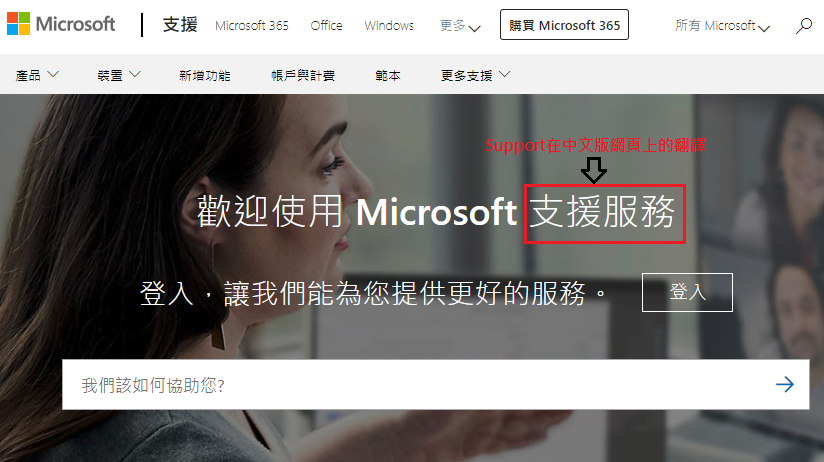
\includegraphics[width= .8\textwidth]{../論文截圖/4-1-9 Page should contain element要驗證的網頁元件.png}
\caption{*Page Should Contain Element 測試腳本要驗證的網頁元件}
\end{figure}

\begin{figure}[H]
\centering
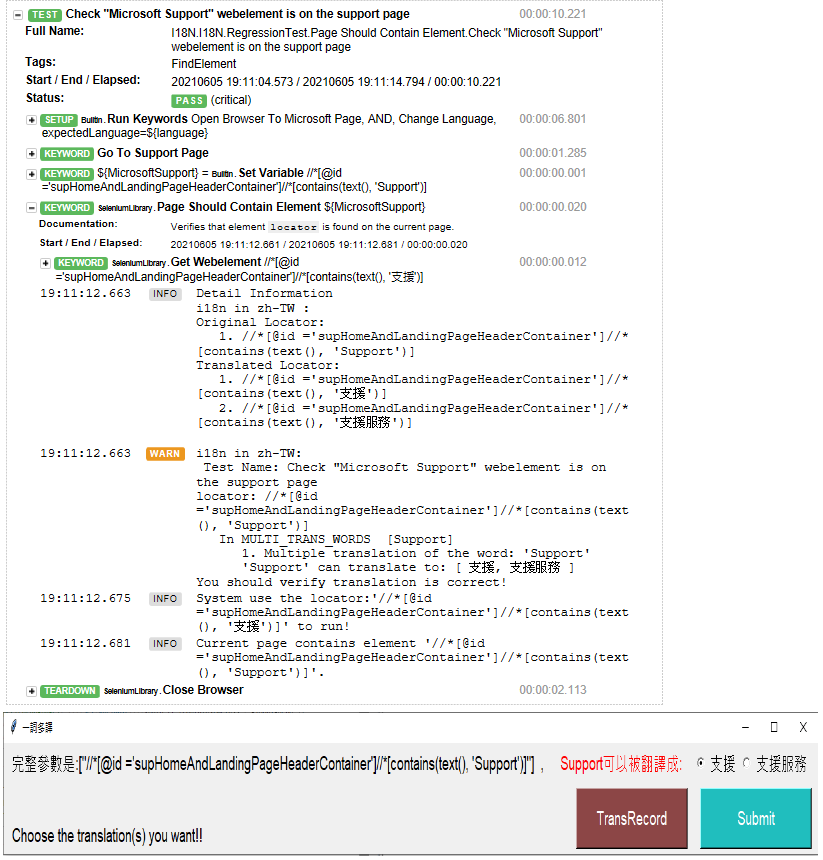
\includegraphics[width= .8\textwidth]{../論文截圖/4.1.5-2 page should contain element 1st run.png}
\caption{*Page Should Contain Element測試腳本第一次執行通過}
\end{figure}
\begin{figure}[H]
\centering
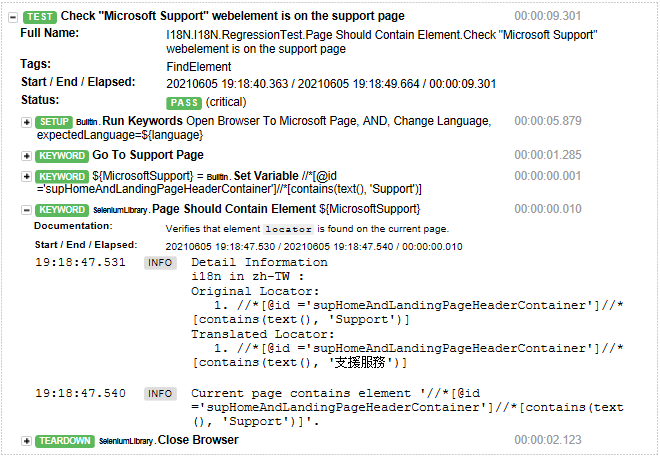
\includegraphics[width= \textwidth]{../論文截圖/4.1.5-3 page should contain element 2nd run.png}
\caption{*Page Should Contain Element測試腳本第二次執行通過}
\end{figure}

\hspace*{\fill} \\
\\ \hspace*{\fill} \\
\\ \hspace*{\fill} \\
\\ \hspace*{\fill} \\
\\ \hspace*{\fill} \\
%4.1.6
\subsection{Table Should Contain}
\begin{figure}[H]
\begin{lstlisting}[language={python}]
*** Settings ***
Resource    ../CommonVariables.txt
Library    SeleniumLibrary
Library    ../self_util.py
Test Setup    Run Keywords    Open Browser    http://localhost:3000    Chrome
...                    AND    Maximize Browser Window
Test Teardown    Close Browser

*** Test Cases ***
Table should contain "Support"
    ${table} =    Set Variable    //*[@id='i18n-table']
    Wait Until Element Is Visible    ${table}    timeout=${shortPeriodOfTime}
    Table Should Contain    ${table}    Support
\end{lstlisting}
\caption{Table Should Contain在代理關鍵字下執行的測試腳本}
\end{figure}
此測試腳本(如圖4.18),會打開I18n Testing Website,之後使用Table Should Contain 驗證畫面上的Support文字(如圖4.19)。第一次測試通過(如圖4.20),代表參數‘Support’有成功被翻譯,且系統將‘支援’當作‘Support’的其中一種翻譯,隨後跳出了一詞多譯UI。之後,使用者選擇了‘支援’當作‘Support’的唯一翻譯。第二次執行測試腳本通過(如圖4.21),且沒有跳出一詞多譯UI,代表參數‘Support’成功被翻譯為使用者前一次的選擇。

\begin{figure}[H]
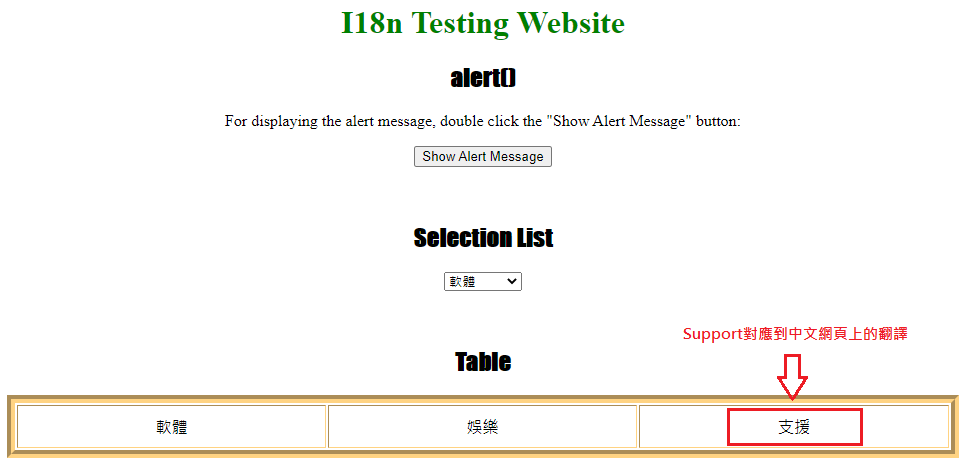
\includegraphics[width= \textwidth]{../論文截圖/4-1-13 Table should contain要驗證的網頁元件.png}
\caption{Table Should Contain 測試腳本要驗證的網頁元件}
\end{figure}

\begin{figure}[H]
\includegraphics[width= \textwidth]{../論文截圖/4.1.6-2 table should contain 1st run.png}
\caption{Table Should Contain 測試腳本第一次執行通過}
\end{figure}

\begin{figure}[H]
\includegraphics[width= \textwidth]{../論文截圖/4.1.6-3 table should contain 2nd run.png}
\caption{Table Should Contain 測試腳本第二次執行通過}
\end{figure}

\hspace*{\fill} \\
\\ \hspace*{\fill} \\
\\ \hspace*{\fill} \\
\\ \hspace*{\fill} \\
\\ \hspace*{\fill} \\
%4-2
\section{改善翻譯邏輯後的驗收測試示例}
以下將舉Page Should Contain Element關鍵字的測試腳本為例,去驗證Microsoft中文官方網頁上的文字。並說明在改善XPath翻譯邏輯前後,執行含有@placeholder屬性的XPath之腳本,將分別得到何種結果。

\begin{figure}[H]
\begin{lstlisting}[language={python}]
*** Settings ***
Resource    ../CommonVariables.txt
Library    SeleniumLibrary
Library    ../self_util.py
Test Setup    Run Keywords    Open Browser To Microsoft Page
...                    AND    Change Language    expectedLanguage=${language}
Test Teardown    Close Browser

*** Test Cases ***
Test web element is on the support page by given special attributes
    Go To Support Page
    ${MicrosoftSupport} =    Set Variable    //*[@id ='supHomeAndLandingPageSearchBox' and @placeholder ='How can we help you?']
    Page Should Contain Element    ${MicrosoftSupport}
\end{lstlisting}
\caption{含有@placeholder屬性的XPath之測試腳本}
\end{figure}

\begin{figure}[H]
\centering
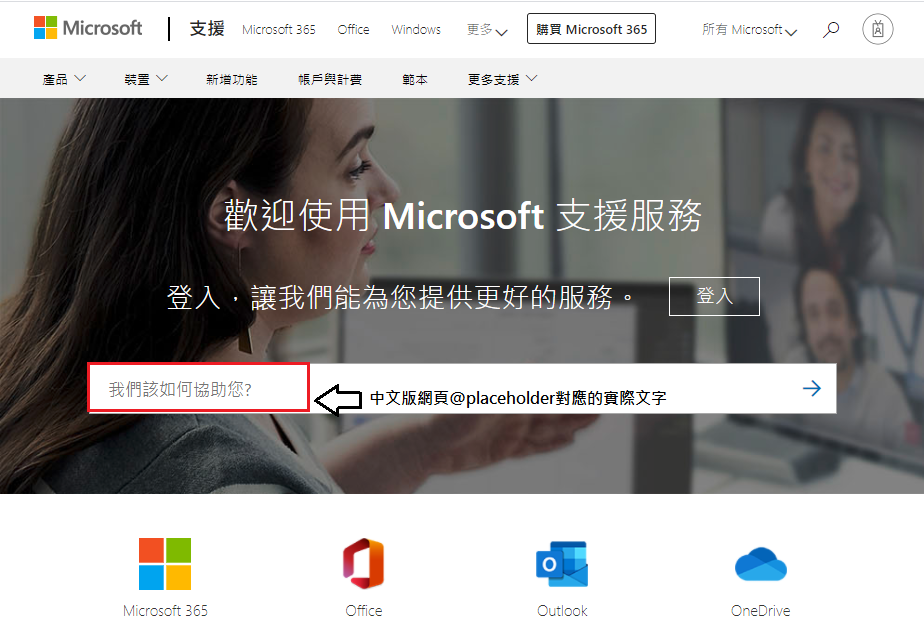
\includegraphics[width= .9\textwidth]{../論文截圖/4-2-2 畫面上@placeholder的實際文字.png}
\caption{中文版Microsoft網頁@placeholder屬性對應的實際文字\cite{microsoft}}
\end{figure}

\begin{figure}[H]
\centering
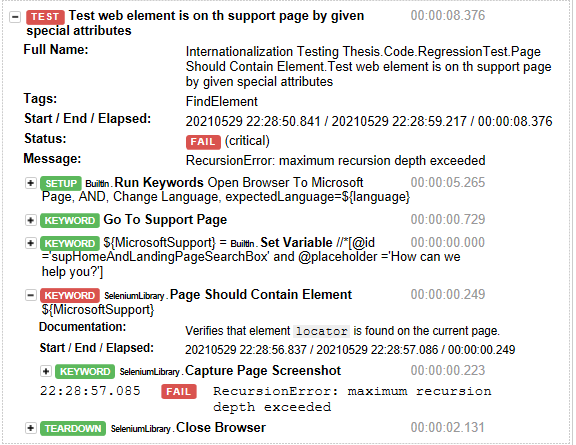
\includegraphics[width= .8\textwidth]{../論文截圖/4-2-3 @placeholder運行在第一版i18n.png}
\caption{待翻譯XPath運行在未改善翻譯邏輯時的i18n工具之結果}
\end{figure}

\begin{figure}[H]
\centering
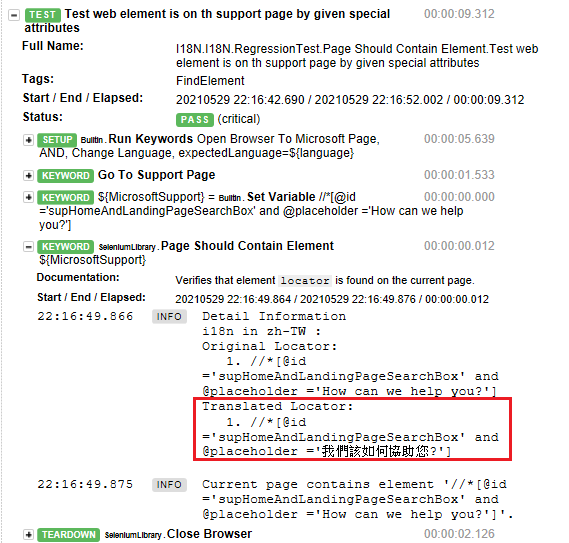
\includegraphics[width= \textwidth]{../論文截圖/4-2-4 @placeholder運行在當前i18n版本.png}
\caption{待翻譯XPath運行在改善翻譯邏輯後的i18n工具之結果}
\end{figure}

由以上的結果我們可以發現,第一版的i18n工具,會因為無法對XPath內的@placeholder屬性做翻譯,而使得測試發生錯誤。本論文新版的i18n工具,因為改善了翻譯邏輯,所以支援各種HTML屬性的翻譯。並成功將”how can we help you?”翻譯為”我們該如何協助您”,進而使測試通過。

%4-3
\section{一詞多譯情況下所產生的圖形化使用者介面}
在遭遇一詞多譯且測試腳本會通過的情況下,以Test should be equal為例(如圖4.26);分別創出兩個變數word1、word2,並用Should Be Equal檢驗兩個變數的值是否正確。測試執行結束後,系統會產生一個圖形化使用者介面(如4.27),上面分別記錄了遭遇一詞多譯的關鍵字完整參數,以及所有可能的翻譯詞,供使用者做選擇。\\

\begin{figure}[H]
\begin{lstlisting}[language={python}]
*** Settings ***
Test should be equal
    ${word1} =    Set Variable    More
    ${word2} =    Set Variable    Support
    Should Be Equal    ${word1}    More
    Should Be Equal    ${word2}    Support
\end{lstlisting}
\caption{Test should be equal 測試腳本}
\end{figure}

\begin{figure}[H]
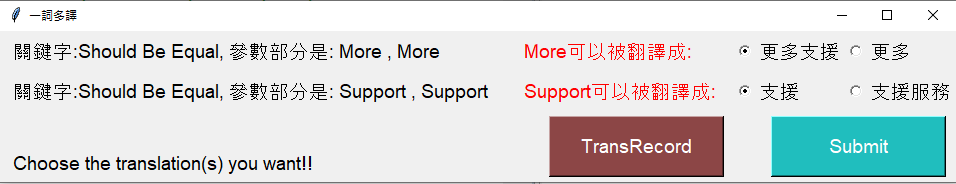
\includegraphics[width= \textwidth]{../論文截圖/4-3-2 測試通過且有一詞多譯時,UI會跳出.png}
\caption{遭遇一詞多譯且測試通過,開啟一詞多譯UI}
\end{figure}

當使用者選擇了希望的翻譯並按下Submit按鈕後,系統便會產生一份設定檔,以利下次執行到同一份腳本的同一關鍵字時,直接套用選擇的翻譯,同時清空一詞多譯介面上的翻譯選項(如圖4.28)。

\begin{figure}[H]
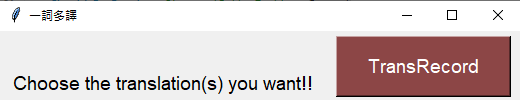
\includegraphics[width= \textwidth]{../論文截圖/4-3-3 選擇翻譯後,清空選項.png}
\caption{按下Submit按鈕後,將翻譯寫進設定檔,同時清除翻譯選項}
\end{figure}

假如使用者選擇錯誤時,則可以點擊TransRecord按鈕來打開翻譯紀錄的介面,上面記錄著使用者曾經的翻譯選擇,並有一顆Undo按鈕(如圖4.29)。使用者選擇了要清除的翻譯紀錄後,按下Undo按鈕,系統便會將設定檔中的該資料刪除,同時關閉翻譯紀錄介面,當再次打開翻譯紀錄介面時,可以發現被選擇清除的資料已消失(如圖4.30)。

\begin{figure}[H]
\centering
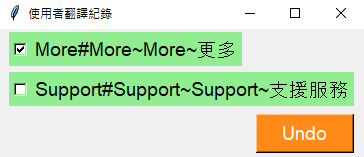
\includegraphics[width= .5\textwidth]{../論文截圖/4-3-4 介面上記錄著使用者翻譯選擇.png}
\caption{打開翻譯紀錄介面,上面記錄著使用者翻譯選擇}
\end{figure}

\begin{figure}[H]
\centering
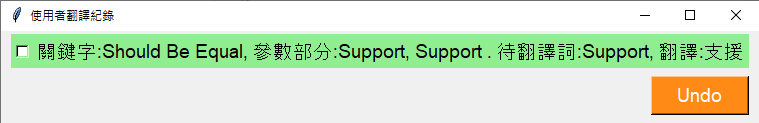
\includegraphics[width= .5\textwidth]{../論文截圖/4-3-5 將選擇的翻譯清除後,再次打開翻譯紀錄介面.png}
\caption{清除選擇的翻譯紀錄後,再次打開翻譯紀錄介面}
\end{figure}

然而,並非所有的測試腳本都會遭遇一詞多譯,且總是通過。因此,底下將分別說明在其他兩種情況下,系統會有甚麼不同的反應:

\begin{itemize}
\item[1.]測試腳本不通過:
若測試腳本不通過,則不論遭遇一詞多譯與否,皆不會跳出一詞多譯UI。其設計想法為,因為系統有檢驗的機制,所以此刻測試腳本不會通過,則代表原先未翻譯前的測試腳本也不會通過。而為原先就會發生錯誤的待翻譯詞選擇其翻譯,對使用者而言,顯然是毫無意義的,但是為了測試結果的完整性,系統還是會於測試報表上顯示一詞多譯的warning資訊(如圖4.31)。
\begin{figure}[H]
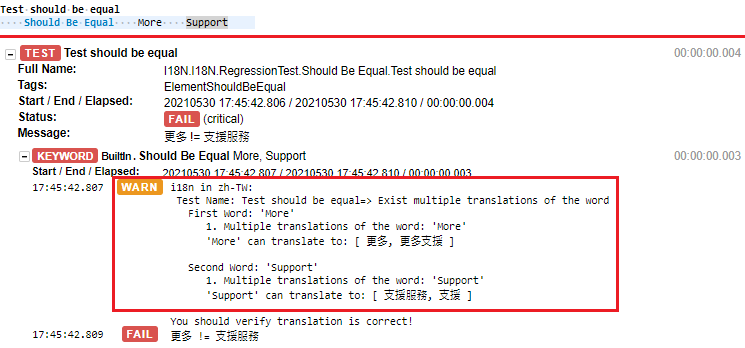
\includegraphics[width= \textwidth]{../論文截圖/4-3-6 測試腳本fail,不跳UI.png}
\caption{測試腳本不通過的情況下,不跳出UI,但會顯示warning資訊於報表}
\end{figure}
\item[2.]測試腳本通過,且沒有遭遇一詞多譯: 
在測試腳本通過且沒有遭遇一詞多譯的情況下,測試結束後便不會跳出一詞多譯UI介面。但有一種情況是,關鍵字的參數部分原本會遭遇一詞多譯,但因為前一次執行時使用者已針對此待翻譯詞選擇了翻譯,所以被系統視為只有一種翻譯,因此不跳出一詞多譯UI(如圖4.32)。(有關系統如何判定翻譯已被使用者選擇,詳見本論文3-2節)
\begin{figure}[H]
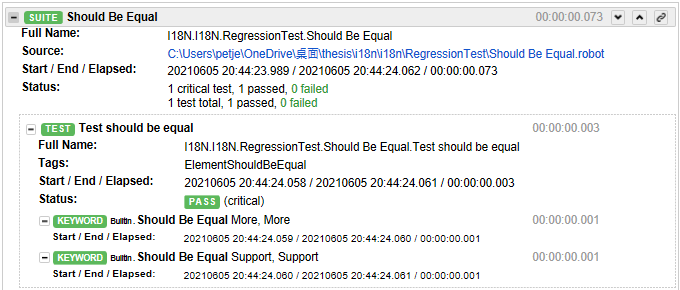
\includegraphics[width= \textwidth]{../論文截圖/4-3-7 測試腳本pass且沒一詞多譯,不跳UI.png}
\caption{測試腳本通過且沒有遭遇一詞多譯的情況下,不跳出UI}
\end{figure}
\end{itemize}

%4-4
\section{使用涵蓋多項代理關鍵字的測試腳本}
以上介紹的測試案例,分別呈現了本論文各項功能改善後的實際成果,但因為都偏向單一關鍵字或單一功能的測試,在此將設計一個較複雜的Robot Framework網頁自動化驗收測試腳本,內部使用到多種代理關鍵字,來對Microsoft的中文版網頁進行一系列操作。同時,會遭遇到一詞多譯,並且會使用相別於第一版i18n所列舉的html待翻譯屬性來撰寫XPath。藉此來對新版i18n工具作一個驗收測試。

以下將執行Test multiple user behaviors on Microsoft website測試腳本兩次,分別呈現選擇一詞多譯翻譯前後,測試結果有何差異之處。

\begin{figure}[H]
\begin{lstlisting}[language={python}]
*** Settings ***
Resource    ./Keywords.txt
Library    SeleniumLibrary
Test Setup    Run Keywords    Open Browser To Microsoft Page
...                    AND    Change Language    expectedLanguage=${language}
Test Teardown    Close Browser

*** Test Cases ***
Test multiple user behaviors on Microsoft website
    Go To Support Page
    Support Button Text Should Be    Support
    Wait Until Element Is Visible    //*[@id = 'uhfCatLogo' ]//*[normalize-space()='Support']
    Click Element    //*[@id = 'uhfCatLogo' ]//*[normalize-space()='Support']
    ${MicrosoftSupport} =    Set Variable    //*[@id ='supHomeAndLandingPageHeaderContainer']//*[contains(text(), 'Support')]
    Page Should Contain Element    ${MicrosoftSupport}

*** Keywords ***
Support Button Text Should Be
    [Arguments]    ${expected}
    ${supportButton} =    Set Variable    //*[@id ='uhfCatLogo']
    Element Text Should Be    ${supportButton}    ${expected}
\end{lstlisting}
\caption{Test multiple user behaviors on Microsoft website測試腳本實作}
\end{figure}
此測試腳本(如圖4.33),會打開Microsoft中文官方網頁,先到支援頁面,之後點擊‘支援’的Logo,到新的支援頁面。最後,驗證畫面上的橫向標語有包含‘支援服務’字樣。因為同時遭遇到3種Support需要被翻譯,系統便會逐一將它們紀錄下來,待測試腳本結束後,分別顯示於一詞多譯UI上。

\begin{figure}[H]
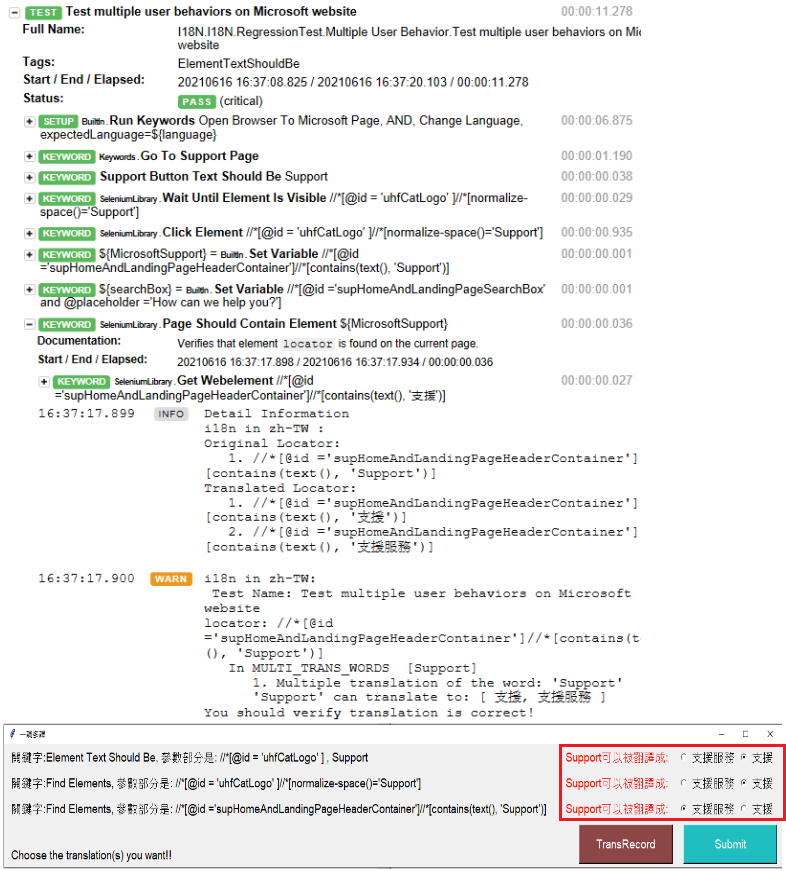
\includegraphics[width= \textwidth]{../論文截圖/4-4-2 test multiple user behaviors測試腳本1st run.png}
\caption{Test multiple user behaviors on Microsoft website測試腳本第一次執行結果}
\end{figure}

第一次執行測試腳本(如圖4.34)結束後,使用者分別為三種不同情況下遭遇一詞多譯的Support,選擇了支援、支援、支援服務為其正確翻譯,並點擊Submit按鈕,將選擇寫入設定檔中。

\begin{figure}[H]
\centering
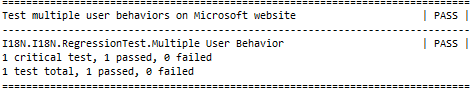
\includegraphics[width= .9\textwidth]{../論文截圖/4-4-3 test multiple user behaviors測試腳本2nd run.png}
\caption{Test multiple user behaviors on Microsoft website測試腳本第二次執行結果}
\end{figure}

第二次執行測試腳本時(如圖4.35),會根據設定檔內的翻譯紀錄,分別對三種Support進行翻譯。因為被系統判定為單一翻譯,所以測試結束後,並不會顯示一詞多譯UI。
